\section{Pioneering Years}
It was in 1959 in Québec, Canada, when I first dealt with a computer. I had
registered in a course on Numerical Analysis, taught by Prof. Goodspeed. But the
computer was not up to the professor's name. In fact, it was not only slow, but
"down", whenever we had concocted a small program as part of an exercise.
Hence, my first encounter with a computer was dismal and discouraging. I cannot
explain how I kept up my interest in computing. But I sensed it would be important
in the future.

The available computer was an Alwac III-3E. It rested on several thousands of
electronic tubes, mostly double triodes, and it occupied a full room. A tube had
typically a life-time of 10'000 hours. Hence, you could reckon that one - and
thereby the entire system - would die every few hours. And it did! Programming
was done by constructing tables of instructions in hexadecimal code. I thought
there was potential for improvement.

My 2nd go at computers was a year later in Berkeley. There was a large IBM 704
computer, one of the first built with transistors instead of tubes, and therefore
much more reliable. It was accessible only via punched card decks delivered to the
Computing Center. Card decks from various customers were piled up by operators,
and the system automatically processed one deck after another. This was called
batch processing. Results could be fetched several hours or even days later on
endless paper as texts consisting of digits and capital letters. Programming was in
the new language Fortran (formula translation). This was a definite improvement
over hexadecimal code, but I could no longer understand how the computer
operated. Again, I felt that there was room for improvement.

In the years 1960-1965 large, remote computers dominated the computing world.
They became called main frames and filled large, air-conditioned rooms. All brands
were more or less the same, differing by word-size, memory size, and, of course,
execution speed. They typically featured one or two accumulator registers. 3 
innovations deserve being mentioned. The 1st is the \emph{index register}, whose
value is added to an operand address during the fetch cycle.

As a representative of these main frames, we very briefly outline the IBM 704. It
featured a memory (store) of 32768 ($=2^{15}$) words of 36 bits each. At the time,
character sets consisted of 64 ($=2^6$) characters; hence, computers featured word
sizes which were multiples of 6 (6-bit bytes!). Numbers were stored in the
sign-magnitude form, a single bit for the sign, 35 bits for the absolute value.
The 704's core consisted of the 36-bit accumulator register (in which supposedly
sums were to be accumulated), the MQ register (holding the multiplier for
multiplications or the quotient for divisions), and 3 15-bit index registers.
There existed 2 instruction formats:
\begin{figure}[h!]
  \centering
  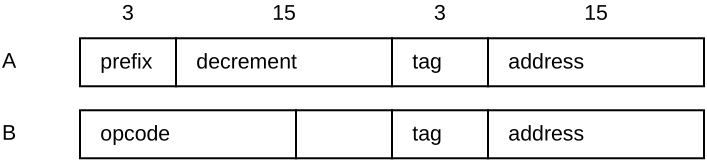
\includegraphics[width=.9\textwidth]{i/1}
\end{figure}
 
Typical type-B instructions were LDA, STA, ADD for loading, storing and adding a
variable (in memory) to the accumulator. The effective address was computed as the
sum of the address field and the index register specified by the tag field. There
were only a few type-A instructions. An example is TIX, implying a transfer to the
given address, and subtraction of the decrement from the specified index register.
This complex instruction was designed to implement fast loops with consecutive
index values.

The 2nd innovation was the \emph{interrupt}, implemented in the later 7090 model.
Here an external signal from an input/output device may cause the interruption of
the current instruction sequence and issue a call of a subroutine, a so-called
interrupt handler. The consequences for programming were considerable.

The 3rd innovation was \emph{floating-point numbers}. There had occurred many heated
discussions on how to represent fractional (real) numbers. The options were fixed-point
and floating point. In the latter case, a (real) number $x$ is represented by 2
integers packed into a single word, say $e$ and $m$, with $x = m B^e$, and $1.0 \le m
< B$. Typically $B = 2$. The 704 took about $80 \mu$s for a floating-point addition,
and $8 \mu$s for an integer addition.

The most numerable main frames were the IBM 704, 7090, 7094, the UNIVAC 1108, and
(a bit later) the CDC 1604 (with 48-bit words and 6 index registers).

Apart from the 704, I encountered in 1961 a much smaller computer available at the
institute led by Prof. Harry Huskey. This was a Bendix G15, designed by Huskey based
on "Turing's computer" at the NPL in England. It was a stand-alone machine, and one
had to sign up time on it by the hour and a few days ahead. It was an ingenious design
with few tubes and a magnetic drum store. It used a serial adder, essentially with a
single tube. Programming consisted of constructing tables of encoded instructions.
What made programming particularly intriguing, or rather cumbersome and tricky, was
that their placement on the drum tracks was of crucial importance for execution speed.
Any word appeared under the reading head only once during a drum revolution, i.e.
about every 40 ms in the worst case. Evidently, the G15 was an interesting device for
puzzle-minded guys, but no pointer to the future. However, I could now fully
understand how such a machine functioned. This is what constitutes progress.
